\section{Chyby měření (rozdělení, výpočet, chyby metody, chyby měřicích přístrojů). Nejistoty měření - typy, výpočet nejistoty A, B, kombinovaná a rozšířená nejistota. Nejistoty nepřímých měření.}
Chyba měřění = přesnost prováděného měření, vyjadřuje se jako rozdíl mezi naměřenou a skutečnou hodnotou měřené veličiny.
\subsection*{Rozdělení}
\begin{itemize}
    \item Chyby měření
          \begin{itemize}
              \item Absolutní
              \item Relativní
          \end{itemize}
    \item Chyba metody
    \item Chyba měřícího přístroje
          \begin{itemize}
              \item Třída přesnosti u analogových měřících přístrojů
              \item Základní chyba číslicových měřících přístrojů
          \end{itemize}
    \item Chyby rušivými vlivy
    \item Podle způsobu výskytu
          \begin{itemize}
              \item systematické
              \item náhodné
              \item hrubé
          \end{itemize}
    \item podle místa vzniku
          \begin{itemize}
              \item Chyby metody měření
              \item Chyba měřícího zařazení
              \item Chyba použitých etalonů
          \end{itemize}
    \item podle příčiny vzniku
          \begin{itemize}
              \item Chyby experimentátora
              \item způsobené rušivými vlivy
              \item vliv přístroje na měřený objekt
          \end{itemize}
\end{itemize}
\newpage
\subsection*{Absolutní chyba měření}
rozdíl mezi naměřenou a kovenčně pravou hodnotou
\begin{equation}
    \Delta_X = X_M - X_P \;\;\;\; [X]
\end{equation}
\subsection*{Relativní chyba měření}
chyba vyjádřená v procentech, častější než absolutní
\begin{equation}
    \delta_X = \frac{\Delta_X}{X_M} \;\;\;\; [\%]
\end{equation}
\subsection*{Korekce}
hodnota, která se musí přičíst k naměřené, aby se získala konvenčně správná hodnota
\begin{equation}
    K_X = X_P - X_M = -\Delta_X \;\;\;\; [X]
\end{equation}
\subsection*{Chyba metody}
vzniká tak, že při výpočtu neuvažujem všechny okolní vlivy nebo zjednodušením/zaokrouhlením výpočtu\\
systematická chyba, která lze eliminovat
\subsection*{Chyba měřícího přístroje}
kalibrací se stanovuje korekční křivka\\
výrobce udává absolutní chybu přístroje\\
\paragraph*{Třída přesnosti pro analogové měřící přístroje}
jedná se o chybu udávanou třídou přesnosti přístroje podle normy ČSN EN 60359(0,05;0,1;0,2;0,3;0,5;1;1,5;2;2,5;3;5)\\
Výpočet třídy přesnosti z maximální absolutní chyby $\Delta_{max}$ na rozsahu $X_R$:
\begin{equation}
    \delta_{TP} = \frac{|\Delta_{max}}{X_R}\cdot 100 \;\;\;\; [\%]
\end{equation}
Jeden přístroj může mět víc tříd nepřesnosti pro různé rozsahy\\
\paragraph*{Vyjadřování chyb číslicového přístroje}
dělí se na:
\begin{itemize}
    \item Základní chybu přístroje
    \item Přídavná chyba přístroje
\end{itemize}
\subparagraph*{Základní chyba}
má dvě složky \\
chyba z měřené hodnoty - nedokonalost nastavení měřících prvků - multiplikativní chyba\\
chyba z rozsahu - posunutí nuly, zbytkové napětí - aditivní chyba\\
Absolutní chyba:
\begin{equation}
    |\Delta_p| = |\Delta_M| + |\Delta_R| = \frac{|\delta_M \cdot X_M|+|\delta_R \cdot X_R|}{100}
\end{equation}
index M - naměřená hodnota \\
index R - rozsah \\
Relativní chyba:
\begin{equation}
    |\delta_p| = |\delta_M| + |\delta_R|
\end{equation}
\\
Způsob zapsání chyby:\\
\textpm(0,05\% z údaje + 0,01\% z rozsahu)\\
\textpm(0,05\% z údaje + 1 digit)
\begin{equation}
    \delta_R = \frac{d}{D}\cdot 100 \;\;\;\;[\%]
\end{equation}
D \dots maximální počet digitů(tj. největší zobrazitelné číslo) \\
d \dots udaný počet digitů posledního místa displeje(většinou 1)\\
\subsection*{Systematické chyby}
přičítá nebo násobí se k měřené hodnotě\\
lze ji určit výpočtem nebo přesnějším měřením\\
lze téměř eliminovat\\

\subsection*{Náhodné chyby}
nelze odstranit korekcí, chová se nepředvídatelně\\
směrodatná odchylka do jisté míry určuje přesnost měření - určuje tvar gaussovy křivky
\begin{equation}
    \sigma = \sqrt{\frac{1}{N}\sum^N_{i=1}(x_i-\overline{x})^2}
\end{equation}
\newpage
\subsection*{Hrubé chyby}
hrubý zásah do procesu měření, výrazně převyšuje rozptyl statistické chyby \\
omyl člověka, výrazná změna podmínek, porucha\\
\begin{figure}[H]
    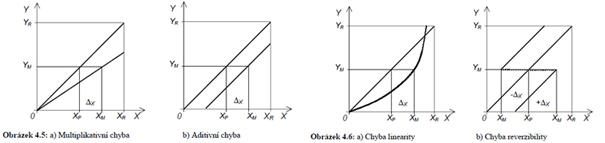
\includegraphics{images/chyby.png}

\end{figure}

\subsection*{Nejistoty}
Parametr přidružený k výsledku měření, který charakterizuje rozptyl hodnot, které by mohly být důvodně přisuzovány k měřené veličině s určitou pravděpodobností.\\
\begin{itemize}
    \item Standartní nejistota typu A
    \item Standartní nejistota typu B
    \item Kombinovaná standartní nejistota
    \item Rozšířená standartní nejistota
    \item Nejistoty pro nepřímá měření
\end{itemize}

\subsubsection*{Standartní nejistota typu A}
Určuje se  z opakovaných měření.\\
zjišťuje se pomocí výběrového rozptylu hodnot.\\
Mírou nejistoty typu A je výběrový směrodatná odchylka výběrového průměru\\
\begin{equation}
    \overline{x} = \frac{1}{n}\sum^n_{i=1}
\end{equation}
\begin{equation}
    u_a(x) = \sqrt{\frac{1}{n(n-1)}\sum^n_{i=1}(x_i-\overline{x})^2}
\end{equation}
\newpage

\subsubsection*{Standartní nejistota typu B}
Nutnost znát všechny zdroje nejistot, které se dají kvalifikovat, tedy určit jinak, než experimentálně.\\
Zdroje nejistot - kalibrace, stabilita přístrojů, dynamické chyby přístrojů, vnitřní tření\\
Vlivy:
\begin{itemize}
    \item vliv metody - ztráty, interakce s měřeným předmětem, nejistoty použitých konstantn, vlastní ohřev, vlivy reálných parametrů oproti ideálním
    \item vliv operátora - nedodržení metodik, elektrostatické pole, tepelné vyzařování
    \item ostatní vlivy - náhodné omyly při odečtu nbo zápisu hodnot, globální vlivy
\end{itemize}
Dají se vypsat z datasheetů nebo odhadovat.\\
Výpočet nejistoty B:
\begin{equation}
    u_{BZ}(x) = \frac{\Delta_{zmax}}{\kappa}
\end{equation}
Celková nejistota typu B je geometrický součet nejistot jednotlivých zdrojů
\begin{equation}
    u_B(x) = \sqrt{\sum^n_{z=1}u^2_{Bz}(x)}
\end{equation}
Koeficient tvaru rozložení $\kappa$ se určuje z tabulky:
\begin{figure}[H]
    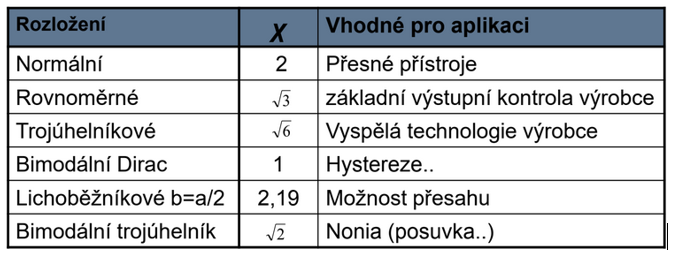
\includegraphics[scale = 1]{images/koef_rozlozeni.png}
\end{figure}
\newpage
Vzorový výpočet nejistoty typu B pro analogový přístroj:
\begin{figure}[H]
    \centering
    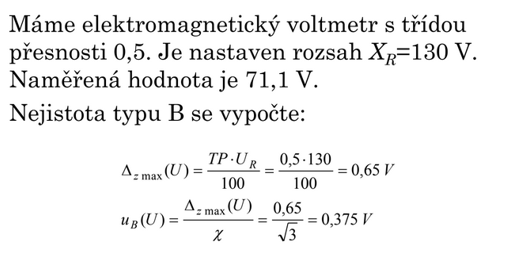
\includegraphics[scale = 1]{images/nejistotaB_analog.png}
\end{figure}
Vzorový výpočet pro nejistotu typu B pro digitální přístroj:
\begin{figure}[H]
    \centering
    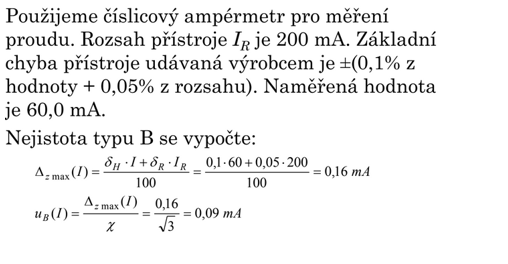
\includegraphics[scale = 1]{images/nejistotaB_digital.png}
\end{figure}

\subsubsection*{Kombinovaná standartní nejistota}
Geometrický součet nejistoty typu A a B
\begin{equation}
    u_C(x) = \sqrt{u_A^2(x)+u_B^2(x)}
\end{equation}
\newpage

\subsubsection*{Rozšířená standartní nejistota}
Kombinovaná standartní nejistota odpovídá intervalu, ve kterém by se výsledky pohybovaly s pravděpodobností 68\%.\\
Rozšířená standartní nejistota pomocí koeficientu tuto pravděpodobnost zvyšuje, koeficient se volí podle tabulky:
\begin{figure}[H]
    \centering
    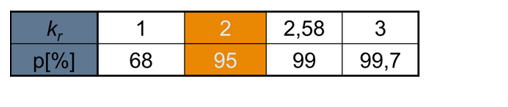
\includegraphics[scale = 1]{images/nejistota_roz.png}
\end{figure}
Nejistota vzniká Kombinovanou standartní nejistotou vynásobenou tímto koeficientem.
\begin{equation}
    U(x) = k_r\cdot u_C(x)
\end{equation}

\subsection*{Nepřímá měření}
Výsledek měření je určen výpočtem na základě známých fyzikálních zákonů z přímých měření vstupních veličin.\\
Výstupní veličina je funkcí průměrných vstupních veličin.\\
\subsubsection*{Nejistota nepřímého měření nekorelovaných vstupních veličin}
Odhad veliiny Y, která je funkcí nekorelovaných vstupních veličin X je dána vztahem:
\begin{equation}
    u(\overline{y}) = \sqrt{\sum^N_{i=1}\left(\frac{\partial f}{\partial X_i}u(\overline{x_i})\right)^2} = \sqrt{\sum^N_{i=1}A_i^2\cdot u^2(\overline{x_i})}
\end{equation}
\begin{equation}
    A_i = \frac{\partial f(X_1,X_2,\dots ,X_N)}{\partial X_i}
\end{equation}
$f$ \dots funkční závislost pro výstupní veličinu $Y$ \\
$A_i$ \dots citlivostní koeficient\\
$u(\overline{x_i})$ \dots nejistota odhadu vstupní veličiny $X_i$\\
\newpage
\subsubsection*{Nejistota nepřímého měření vzájemně korelovaných vstupních veličin}
Odhad veličiny $Y$, která je funkcí vzájemně korelovaných vstupníc veličin $X$, zahrnuje rovněž kovariance mezi jednotlivými odhady vstupních veličin a ty rovněž přispívají k výsledné nejistotě podle vztahu:
\begin{equation}
    u(\overline{y}) = \sqrt{\sum^N_{i=1}A_i^2\cdot u^2(\overline{x_i})+2\sum^N_{i=2}\sum^{N-1}_{k<i}A_i\cdot A_k \cdot u^2(\overline{x_i},\overline{x_k})}
\end{equation}
$u(\overline{x_i},\overline{x_k})$ \dots kovariace mezi navzájem korelovanými odhady vstupních veličin $\overline{x_i},\overline{x_k}$


\section{Analogově-číslicové převoddníky pro měřicí techniku - rozdělení, princip základních typů AD převodníků, vlastnosti, použití}
Převod analogové diskrétní proměnné veličiny(napětí) na diskrétní údaj vyjádřený číslem.\\
Diskretizace analogového signálu:
\begin{itemize}
    \item V amplitudě - kvantování
    \item V čase - vzorkování(vzorkovací teorém - vzorkovací frekvence musí být větší, než 2* maximální požadovaná přenášená frekvence)
    \item Kódování
\end{itemize}
Kvantizační chyba - chyba zaokrouhlování na nejmenší jednotku přístroje. Při časové změně měřené veličiny vzniká kvantovací šum\\
\begin{figure}[H]
    \centering
    \includegraphics*[scale = 1]{images/adc_prevodni_char.png}
    \caption*{Převodní charakteristika měřicího přístroje}
\end{figure}
$K_i$ ideální převodní charakteristika\\
$K_S$ je skutečná převodní charakteristika\\
Chyby, které se vyskytují:
\begin{itemize}
    \item chyba nuly - nenulový výstup pro nulové napětí
    \item chyba konstanty - jiný sklon charakteritiky
    \item chyba linearity - průměrná charakteristika není lineární
\end{itemize}
\newpage
Kritéria hodnocení AD převodníku:
\begin{itemize}
    \item rozlišovací schopnost
    \item krok kvantování
    \item chyba kvantování
    \item rychlost převodu
    \item přesnost
    \item stabilita
\end{itemize}
\subsection*{Rozdělení AD převodníků}
\begin{itemize}
    \item Komparační
          \begin{itemize}
              \item Metoda paralelního porovnání
              \item Metoda sérioparalelního porovnání
          \end{itemize}
    \item Kompenzační
          \begin{itemize}
              \item Kompenzační metoda
              \item Metoda postupné aproximace
          \end{itemize}
    \item Integrační
          \begin{itemize}
              \item Integrační metoda (metoda dvojté integrace)
              \item Převod napětí na kmitočet metodou jednoduché integrace
          \end{itemize}
    \item Sigma-delta modulace
\end{itemize}

\subsection*{Komparační A/D převodník(FLASH)}
Srovnává měřené napětí s různě nastavenýma hodnotama referenčního napětí najednou.\\
Vzorkovací frekvence desítky MHz až 3 GHz\\
krátká doba převodu(ns) - nejrychlejší\\
drahý, není odolný vůči sériovému rušení
\begin{figure}[H]
    \includegraphics*[scale = 1.3]{images/adc_komparacni.png}
\end{figure}
\newpage
\subsection*{Kompenzační A/D převodník}
měřené konstantní napětí se porovnává se známým stavitelným kompenzačním napětím - nastavuje se tak, aby se blížilo měřenému\\
nejde nastavit naprostá shoda, maximálně zanedbatelný rozdíl - nastavuje se postupně\\
Typy:
\begin{itemize}
    \item Přírůstkový převodník
    \item Sledovací převodník - umožňuje čítat i dolů
    \item Aproximační převodník - nahrazen registrem
\end{itemize}
\subsubsection*{Metoda postupné aproximace}
Hodnota napětí vyjádřena přirozeným binárním číslem\\
při převodu se určuje bit po bitu od největšího po nejmenší\\
8-16 bitové\\
vzorkovací frekvence 10kHz - 3MHz\\
\begin{figure}[H]
    \includegraphics*[scale = 1]{images/adc_kompenzacni_aprox.png}
\end{figure}
\newpage

\subsection*{Integrační A/D převodník}
vhodné a často používané pro číslicové voltmetry\\
výsledkem integrace je střední hodnota\\
Parametry:
\begin{itemize}
    \item 10-27 bitové
    \item vzorkovací frekvence 0,1Hz až 1kHz
    \item pomalé
    \item velká přesnost, eliminace sériového rušení
\end{itemize}
Princip:
\begin{itemize}
    \item dvojí(dvoutaktní) integrace
    \item neznámé vstupní napětí porovnáváno s referenčním opačné polarity
    \item po skončení druhého taktu stav čítače hodinových pulsů N udává velikost neznámého napětí
\end{itemize}

\begin{equation}
    N = f_hT_2 = f_hT_1\cdot \frac{U_{vst}}{Z_{REF}} = N_c \cdot \frac{U_{vst}}{Z_{REF}}
\end{equation}
\begin{figure}[H]
    \includegraphics*[scale = 1]{images/adc_integrac.png}
\end{figure}

\subsubsection*{Převodník napětí na kmitočet}
Převod měřeného napětí na kmitočet a ten pak změřit číslicově.\\
převáděné napětíje trvale připojeno na vstup integrátoru, vyvolává změnu napětí na výstupu integrátoru, které se v komparátoru porovnává s konstantním napětím\\
při překročení hodnoty se změní na opačné výstupní napětí integrátoru\\
kmitočet výstupních impulsů je pak úměrný měřenému napětí
\begin{figure}[H]
    \includegraphics*[scale = 1]{images/adc_V_na_f.png}
\end{figure}

\subsection*{Sigma-delta modulace}
Dle taktu Uc vzorkování na komparátor\\
Uo obdelníkové, dle trvání vyšší a nižší hodnoty vyjadřuje Ux\\
dobré rozlišení o na 16 bit při 100kHz, dlouhá odezva
\begin{figure}[H]
    \includegraphics*[scale = 1]{images/adc_sigma_delta_schema.png}
\end{figure}

\begin{figure}[H]
    \includegraphics*[scale = 1]{images/adc_sigma_delta_graf.png}
\end{figure}


\subsection*{Vlastnosti}
\begin{itemize}
    \item Rozlišovací schopnost - dána počtem rozlišitelných úrovní analogového signálu. Pro n-bitový převodník je to $2^n$ úrovní
    \item Krok kvantování(citlivost) - rozdíl dvou hodnot vstupního analogového napětí, kdy nastává přechod od jednoho číslicového výstupu k druhému
    \item Chyba kvantování - maximální rozdíl mezi hodnotou analogové veličiny a hodnotou odpovídající danému ódovanému slovu(obvykle polovina kroku kvantování)
    \item Rychlost převodu
    \item Přesnost - dána chybou převodníku
    \item Stabilita - vyjadřuje stálost převodníku při působení různých rušivých vlivů
\end{itemize}

\subsection*{Použití}
Zpracování analogových signálů v digitálních přístrojích.

\section{Měření napětí a proudu. Změna rozsahů voltmetru a ampérmetrů. Rušení u měřicích přístrojů.}

\subsection*{Měření napětí}
\subsubsection*{voltmetry}
zapojení paralelně k zátěži\\
ideální voltmetr - nekonečný vnitřní odpor, reálně digitální 10MOhm, analogový 5kOhm/V \\
\subsubsection*{Přístroje pro měření napětí}
\begin{itemize}
    \item analogové
          \begin{itemize}
              \item reagují na hodnotu měřeného napětí výchylkou ručky
              \item obsahují převodník pro změny rozsahů
          \end{itemize}
    \item analogové elektronické
    \item číslicové(stejnosměrný voltrmetr je základem multimetru)
\end{itemize}
\subsubsection*{Měření stejnosměrného napětí(DC)}
na DC napětí se převádí pomocí měřicích převodníků všechny ostatní měřené veličiny\\
v praxi bývá problém s napěťovým offsetem a jeho driftem v jednosměrných předzesilovačích ve voltmetrech\\
u měření vysokých napětí(v řádu kV) problém s bezpečností a izolačními možnostmi materiálu\\
\subsubsection*{Měření střídavého napětí(AC)}
požadovaný parametr obvykle efektivní hodnota\\
Dělí se podle šířky pásma:
\begin{itemize}
    \item Úzkopásmové - selektivní, místo voltmetrl obvykle spektrální analyzátor, oblast vysoké frekvence
    \item Širokopásmové - nejpoužívanější, oblast nízké frekvence (v řádu Hz až kHz)
    \item Multimetry - napěťové rozsahy od mV po stovky V
\end{itemize}
\newpage

\subsubsection*{Měřicí transformátory napětí}
k převodu měřené veličiny na velikost vhodnou k měření a ke galvanickému oddělení měřicích obvodů a přístrojů od vysokého napětí
Transformační poměr pro idealizovaný stav:
\begin{equation}
    p_U = \frac{U_1}{U_2} = \frac{N_1}{N_2}
\end{equation}
\begin{figure}[H]
    \centering
    \includegraphics*[scale = 2]{images/napeti_transformator.png}
\end{figure}
Princip:
\begin{itemize}
    \item primární vinutí M-N se připojuje (MTN-měřicí transformátor proudu)do obvodu paralelně
    \item sekundární vinutí m-n obsahuje měřicí obvod představující vysokou impedanci
    \item MTN musí pracovat v blízkosti stavu narpázdno
    \item se chová jako zdroj s malým vnitřním odporem
\end{itemize}
Vlastnosti:
\begin{itemize}
    \item oproti předřadným odporům velmi malá spotřeba
    \item hodnota sekundárního napětí obvykle 100V
    \item způsobují chybu převodu - udává se třídou přesnosti
    \item způsobují chybu fáze - nutno počítat při měření výkonu
    \item nelze použít, kde by docházelo k magnetování jádra stejnosměrnou složkou průběhu - bo cívky
\end{itemize}
\subsubsection*{Typy rušení}
Na vstupní svorky stejnosměrného voltmetru se mohou k měřenému napětí přičítat rušívá napětí.\\
Rušivá napětí:
\begin{itemize}
    \item Stejnosměrná
    \item Střídavá
    \item Náhodná
\end{itemize}
Nejčastěji rušení střídavé od napájecí sítě s frekvencí 50 Hz.\\
\newpage
Sériové rušení:
\begin{itemize}
    \item Zdroj rušivého signálu je zapojený sériově s měřenou veličinou
    \item Sčítá se s měřeným
\end{itemize}
Odstrańnuje se buď účinným filtrem dolní propusti před číslicovým voltmetrem, nebo některé A/D převodníky dokáží sériové rušení potlačit automaticky.\\
Souhlasné rušení:
\begin{itemize}
    \item při měření napětí mezi dvěma body elektrického obvodu mohou nastat situace, kdy tyto body mají proti společné svorce určité napětí
    \item je vyvoláno rozdílem potenciálu země voltmetru a země měřeného objektu
    \item potlačuje se konstrukcí přístroje - rozpojením zemní smyčky použitím multimetru s bateriovým nanápajením
\end{itemize}

\subsubsection*{Číslicové voltmetry}
Základní měřicí přístroj v praxi, víc se ale využívají multimetry\\
Základní části číslicového voltmetru:
\begin{figure}[H]
    \includegraphics*[scale = 1.5]{images/cislicovy_voltmetr.png}
\end{figure}
Vstupní část umožňuje volbu dílčích měřicích rozsahů. Převádí velkost měřeného napětí na velikost vyhovujícího převodníku napětí na číslo.\\
Dočasné uchování naměřených dat.\\
Parametry:
\begin{itemize}
    \item počet míst zobrazovače (3 až 8\textonehalf)
    \item počet měřicích rozsahů (4 až 6, zkl. rozsah 1 nebo 10V)
    \item přesnost
    \item rozlišovací schopnost - velikost napětí na vstupu voltmwtru, která způsobí změnu údaje voltmetru o 1 na posledním místě číslicového zobrazovače při nejnižším rozsahu
    \item maximální měřené napětí - obvykle 1000 V DC a 750 V AC
    \item rychlost měření
    \item časová stálost
    \item odolnost proti rušení
    \item vstupní impedance
    \item typ použitého AD převodníku
    \item kmitočtový rozsah(50kHz až 2 MHz)
\end{itemize}

Chyby číslicových měřicích přístrojů:
\begin{itemize}
    \item pevné chyby - nezávislé na velikosti vstupního signálu(vyjařují se v \% z měřicícho rozsahu), chyby způsobené:
          \begin{itemize}
              \item Driftem napěťové nesymetrie vstupního zesilovače
              \item Vnitřním šumem přístroje
              \item Zbytkovým napětím spínačů
              \item Chyba kvantováním
          \end{itemize}
    \item Chyby úměrné měřené hodnotě(projevují se multiplikativně, taky v \% z rozsahu) - způsobené chybami:
          \begin{itemize}
              \item přenosu zesilovačů
              \item vstupní děliče
              \item napětí referenčního přístroje
          \end{itemize}
\end{itemize}
Změna rozsahu voltmetru:\\
Rozsah se zvětší zapojením předřadného rezistoru do série - předřadník:\\
\begin{figure}[H]
    \includegraphics*[scale = 1.5]{images/predradnik.png}
\end{figure}

\subsection*{Měření proudu}

Pomocí ampérmetrů - zapojení do série s měřeným obvodem.\\
Ideální ampérmetr má nulový opor, když nějaký má, je to chyba metody.\\
Velikost měřených proudů:
\begin{figure}[H]
    \includegraphics*[scale = 1.2]{images/Imereni.png}
\end{figure}
Měření v rozsahu $\mu A$ až jednotek A.\\
U nižších proudů problém se vstupními proudy a jejich driftem v předzesilovači.\\
U vyšších proudů problém se snímáním proudu, lze použít speciální proudové sondy a nepřímé metody.\\
\newpage

\subsubsection*{Měření malých proudů}
Je potřeba použít měřící zesilovače nebo použít převodník proudu na napětí.\\
To umožňuje měření malých proudů bez úbytku napětí, vstupní odpor se bíží 0 Ohm, bývají součástí číslicových ampérmetrů.\\
Velmi malé proudy se převádí pomocí velkého odporu napětí, které se měří mikrovltmetrem s modulačním zesilovačem.\\
\subsubsection*{Měření velkých proudů}
Proudový transformátor:
\begin{itemize}
    \item pouze pro střídavý proud
    \item úzký frekvenční rozsah
    \item levné, jednoduché
\end{itemize}
Hallova sonda - polovodičový snímač magnetického proudu
\begin{figure}[H]
    \includegraphics*[scale = 1]{images/hallova_sonda.png}
\end{figure}

Vlastnosti:
\begin{itemize}
    \item použití pro DC aj AC proud
    \item rozsah měřených proudů od mA po stovky kA
    \item do frekvence 25 kHz
    \item přesnost až 1\%
    \item digitální výstup
    \item vyšší cena
\end{itemize}
\newpage
Měřicí transformátor proudu\\
princip:
\begin{itemize}
    \item primární obvod měřicícho transformátoru proudu(MTP) je zapojen do série se zdrojem
    \item sekundární vinutí se uzavirá přes měřicí přístroj
\end{itemize}
\begin{figure}[H]
    \includegraphics*[scale = 1.3]{images/proud_transformator.png}
\end{figure}

Měřicí transformátor proudu musí vždy pracovat v blízkosti stavu nakrátko.
\begin{itemize}
    \item před odpojením měřicích přístrojů je nutné sekundární vinutí zkratovat
    \item protéká-li primárním vinutím proud, nesmí být sekundární vinutí rozpojeno
\end{itemize}

Parametry:
\begin{itemize}
    \item transformační poměr
    \item jmenovitá hodnota sekundárního proudu
    \item povolená sekundární zátěž
\end{itemize}
Charakteristické údaje:
\begin{itemize}
    \item Dynamický proud MTP - největší amplituda zkratového proudu při sekundárním vinutí nakrátko - nesmí dojít k mechanickému nebo elektrickému poškození
    \item Tepelný proud - efektivní hodnota primárního proudu po dobu 1 sekundy při sekundárním vinutí nakrátko - nesmí dojít k poškození, závisí na průřezu primárního vinutí
    \item Nadproudové číslo - násobek jmenovitého proudu, kdy chyba převodu dosáhne 10\% při jmenovité zátěži a účiníku
\end{itemize}
Přesnost převodu závisí na:
\begin{itemize}
    \item velikosti měřeného proudu
    \item kmitočtu měřeného proudu
    \item tvaru a vlastnostech jádra a vinutí
    \item velikost a charakteru sekundární impedance
\end{itemize}
Parazitní vlivy:
\begin{itemize}
    \item rozptylová indukčnost obou vinutí
    \item ztráty v železe vlivem vířivých proudů
\end{itemize}
\newpage
Výhody:
\begin{itemize}
    \item lze transformovat nejen z větší na menší
    \item spotřeba měřicích obvodů se s měřicími transformátory nemění se změnou rozsahu
\end{itemize}
Nevýhoda - nelze transformovat střídavé průběhy se stejnosměrnou složkou

Měření proudu pomocí multimetru:
\begin{itemize}
    \item převod proudu na napětí - požadavek co nejmenší impedance
    \item typy převodníků:
          \begin{itemize}
              \item pasivní převodník - přesný snímací rezistor, přepočet měřeného proudu podle poměrů vstupního odporu ampérmetru a bočníku
              \item aktivní převodník - využití OZ
          \end{itemize}
\end{itemize}

\subsection*{Rušení u měřicích přístrojů}
\subsubsection*{Mechanické vlivy}
\begin{itemize}
    \item tření - zvětšením direktivního momentu spirálových pružin, větší spotřeba, menší citlivost přístroje
    \item Otřesy - dát přístroj na měkkou podložku
    \item poloha přístroje - měly by se používat jen v poloze uvedené v seznamu
\end{itemize}

\subsubsection*{Teplota}
\begin{itemize}
    \item Mění se odpor měřicích cívek, předřadníků či bočníků a magnetická indukce permanentních magnetů
    \item předřadníky a bočníky dáváme do přední části přístroje, aby neovlivňovaly měčicí cívky, použijeme materiál, který má nepatrnou závislost na teplotě, chladící otvory
\end{itemize}
\subsubsection*{Vnější elektromagnetické pole}
\begin{itemize}
    \item působí zejména na přístroje, které pracují s vlastním slabým polem
    \item bráníme stíněním měřicího ústrojí krytem z feromagnetického materiálu
\end{itemize}

\subsubsection*{Kmitočet}
\begin{itemize}
    \item změna kmitočtu způsobí změnu údaje u těch přístrojů, jejichž pohybový moment na kmitočtu závisí
    \item u každého přístroje se řeší individuálně
\end{itemize}
\newpage

\section{Měření výkonu v jednofázové a třífázové soustavě. Wattmetry - princip, typy vlastnosti.}
Výkon stejnosměrného proudu:
\begin{equation}
    P = U\cdot I \;\;\;\; [W]
\end{equation}
Výkon střídavého proudu:
\begin{itemize}
    \item Okamžitý výkon(časový okamžik) $p(t) = u(t)\cdot i(t)$   [W]
    \item střední hodnota výkonu(časový interval) $P = \frac{1}{T}\int_0^Tp(t)dt = \frac{1}{T}\int_0^Tu(t)\cdot i(t)dt$    [W]
\end{itemize}

Výkon harmonického proudu a napětí s fázovým posuvem:
\begin{itemize}
    \item Činný výkon    $P = U\cdot I \cdot cos \upvarphi $    [W]
    \item Jalový výkon   $Q = U\cdot I \cdot sin \upvarphi $    [VAr]
    \item Zdánlivý výkon  $S = U \cdot I$                     [VA]
\end{itemize}
Výkon neharmonických proudů a napětí: $P = U_0\cdot I_0 + \sum^{k=n}_{k=1}U_k\cdot I_k \cdot cos \upvarphi_k$     [W]
\subsection*{Měření výkonu v jednofázové soustavě}
Metody:
\begin{itemize}
    \item elektromechanické wattmetry s elektrodynamickým ústrojím
    \item elektronické wattmetry - nejde odečíst proud/napětí na zátěži, přidává se voltmetr/ampermetr
    \item měření třemi voltmetry
    \item měření třemi ampérmetry
\end{itemize}

\subsubsection*{Metoda wattmetrem}
dva způsoby, oba zatíženy chybou metody
\begin{figure}[H]
    \includegraphics*[scale = 1]{images/wattmetry2.png}
\end{figure}
\newpage

\subsubsection*{Metoda třemi voltmetry}
Nepřímá metoda pro měření malých činných výkonů na malých impedancích zátěže Z
\begin{figure}[H]
    \includegraphics*[scale = 1.5]{images/voltrmetry3.png}
\end{figure}

\subsubsection*{Metoda třemi ampérmetry}
\begin{figure}[H]
    \includegraphics*[scale = 1.5]{images/ampermetry3.png}
\end{figure}

\subsubsection*{Měření jalového výkonu}
\begin{figure}[H]
    \includegraphics*[scale = 1.3]{images/jalovec.png}
\end{figure}
Charakter zátěže spotřebiče:
\begin{itemize}
    \item Induktivní - kladný jalový výkon
    \item Kapacitní - záporný jalový výkon
\end{itemize}

\subsubsection*{Měření zdánlivého výkonu}
Jedině nepřímo, počítá se z proudu a napětí


\subsection*{Měření výkonu v třífázové soustavě}
Všechna zapojení vyžadují znalost sledu fází:
\begin{figure}[H]
    \includegraphics*[scale = 1.2]{images/fazovyDiagram.png}
\end{figure}
Sled fází je určem pořadím, v němž veličiny trojfázové soustavy nabývají svého maxima.\\

Fázové napětí - napětí mezi fázovým a nulový vodičem\\
Sdružené napětí - napětí mezi dvěma fázovými vodiči
\begin{figure}[H]
    \includegraphics*[scale = 1.2]{images/sdruzeneNapeti.png}
\end{figure}

\subsubsection*{Základní pojmy}
\begin{itemize}
    \item Souměrná zátěž - Síť je zatížena souměrným spotřebičem, protéká v každé fázi stejný proud(motor)
    \item Nesouměrná zátěž - spotřebič odebírá v každé fázi jiný proud(oblouková pec)
    \item Obecná (nesymetrická) soustava - má obecné velikosti fázových napětí a obecné úhly mezi nimi - čtyřvodičová má přístupný nulový vodič, třívodičová ne
    \item Symetrická soustava - zvláštní případ obecné soustavy, fázová napětí mají stejnou velikost i úhel, sdružené napětí je $\sqrt{3}$ krát větší, než fázové
\end{itemize}

\subsubsection*{Matematický popis}
Souměrná soustava:
\begin{itemize}
    \item efektivní hodnota: $U_1 = U_2 = U_3 = U_f$
    \item fázový posuv: $\upvarphi = 2\pi /3$
\end{itemize}
$u_1 = \sqrt{2}U_fsin(\omega t +\upvarphi)$\\
$u_2 = \sqrt{2}U_fsin(\omega t -120\degree +\upvarphi)$\\
$u_3 = \sqrt{2}U_fsin(\omega t -120\degree +\upvarphi)$\\


Volba  metody záleží na tom, jestli je měřená zátěž ne/symetrická a jestli je trojfázová síť tří nebo čtyřvodičová\\

\subsubsection*{Blondelův teorém}
V n-vodičové soustavě se činný výkon zátěže správně měří nejméně n-1 wattmetry

\subsubsection*{Symetrická zátěž, čtyřvodičová symetrická soustava}
\begin{figure}[H]
    \includegraphics*[scale = 1.2]{images/sym_4_sym.png}
\end{figure}


\subsubsection*{Symetrická zátěž, třívodičová symetrická soustava}
\begin{figure}[H]
    \includegraphics*[scale = 1.2]{images/sym_3_sym.png}
\end{figure}

\subsubsection*{Neymetrická zátěž, čtyřvodičová soustava}
\begin{figure}[H]
    \includegraphics*[scale = 1.2]{images/nesym_4.png}
\end{figure}
\newpage

\subsubsection*{Nesymetrická zátěž, třívodičová soustava}
\begin{figure}[H]
    \includegraphics*[scale = 1.2]{images/nesym_3.png}
\end{figure}

\subsubsection*{Aronovo zapojení}
Slouží k měření rinného výkonu v třívodičové soustavě bez středového vodiče.\\
Lze použít pro souměrnou i nesouměrnou zátěž.\\
Napěťové obvody wattmetrl jsou připojeny na sdružená napětí.
\begin{figure}[H]
    \includegraphics*[scale = 1.2]{images/Aron.png}
\end{figure}

\subsubsection*{Měření Jalového výkonu}
Nutnost zajistit zpoždění fázoru napětí na napěťové cívce každého wattmetru o 90° oproti fázoru napětí při měření činného výkonu - připojit sdružená napětí na napěťové cívky\\
\begin{figure}[H]
    \includegraphics*[scale = 1]{images/jalonen.png}
\end{figure}
\newpage

\subsection*{Wattmetry}
\begin{figure}[H]
    \includegraphics*[scale = 1]{images/wattSchemata.png}
\end{figure}
Rozdělení:
\begin{itemize}
    \item Z funkčního hlediska:
          \begin{itemize}
              \item Průchozí - zapojuje se mezi zdroj a zátěž, měří výkon předávaný zdrojem do zátěže
              \item Pohlcovací - měří výkon předávaný zdrojem do odporové zátěže obsažené ve wattmetru připojeného ke zdroji
          \end{itemize}
          \begin{figure}[H]
              \includegraphics*[scale  = 1]{images/wattTypy.png}
          \end{figure}
    \item Podle způsobu měření a charakteru údaje:
          \begin{itemize}
              \item Analogové
              \item Digitální
          \end{itemize}
\end{itemize}

\subsubsection*{Průchozí wattmetr}
Použití:
\begin{itemize}
    \item nízkofrekvenční oblast
    \item měření harmonických průběhů - energetika
    \item měření neharmonických průběhů - měření výkonu i harmonicky zkresleného průběhu v síti
\end{itemize}


\begin{figure}[H]
    \includegraphics*[scale  = 1]{images/wattPruchozi.png}
\end{figure}

Rozdělení:
\begin{itemize}
    \item Analogové wattmetry
    \item Číslicové wattmetry s analogovým zpracováním signálů
    \item Číslicové wattmetry s číslicovým zpracováním signálů
\end{itemize}

Analogový wattmetr:
\begin{figure}[H]
    \includegraphics*[scale  = 1.3]{images/wattAnalog.png}
\end{figure}

Číslicový wattmetr s analogovým zpracováním signálu
\begin{itemize}
    \item Smodulační násobičkou
          \begin{itemize}
              \item chyba v desetinách procenta
              \item frekvenční pásmo 0-10kHz
              \item Princip:
                    \begin{figure}[H]
                        \includegraphics*[scale  = 1]{images/wattAnalogPrincip.png}
                    \end{figure}
          \end{itemize}
          \newpage

    \item Hallova násobička
          \begin{itemize}
              \item Působí-li na plochu destičky z polovodičového materiálu magnetické pole o indukci B a protéká-li destičkou proud i, objeví se na zbývajících hranách hallovo napětí $U_H$
              \item Napětí $U_H$ je nutno integrovat, abychom získali stejnosměrnou hodnotu úměrnou činnému výkonu P
          \end{itemize}
\end{itemize}
\begin{figure}[H]
    \includegraphics*[scale  = 1.3]{images/wattHallovaNasobicka.png}
\end{figure}

Číslicový wattmetr s číslicovým zpracováním signálu
\begin{itemize}
    \item přechod od předchozího typu doplněný o AD převodník a nahrazení analogové násobičky procesorem
\end{itemize}
\begin{figure}[H]
    \includegraphics*[scale  = 1.3]{images/wattCislicovySchema.png}
\end{figure}

\subsubsection*{Pohlcovací wattmetry}
Určeny k měření výkonu dodávaného zdrojem do odporové zátěže představované samotným wattmetrem.\\
Výkon se určuje buď z napětí na zátěži, nebo z tepelného účiníku.\\
Rozsah MHz až destíky GHz.\\
Většinou ve formě externích modulů k PC nebo jako doplněk spektrálních analyzátorů.\\
Analogový nebo číslicový údaj.\\
Odporová zátěž:
\begin{itemize}
    \item Měřicí rozsah $1 \mu W$ až $1 kW$
    \item pro vyšší frekvence se používá zatěžovací rezistor zakončující koaxiální vedení
\end{itemize}
\begin{figure}[H]
    \includegraphics*[scale  = 1.3]{images/wattOdporovaZatez.png}
\end{figure}

Voní zátěž:
\begin{itemize}
    \item pro střední a větší výkony(desítky W až kW) - přivedený měřený výkon protékající vodu ohřívá, měří se průtok a oteplení vody
    \item buď v koaxiálním provedení(do 3 GHz) nebo vlnovodném provedení(nad 2GHz)
\end{itemize}
\begin{figure}[H]
    \includegraphics*[scale  = 1]{images/wattVodniZatez.png}
\end{figure}

Zátěž v podobě vedení:
\begin{itemize}
    \item Pro měření menších výkonů(desítky W)
    \item použití "suché" zátěže ve formě bezodrazného zakončení koaxiálního vedení nebo vlnovodného vedení
    \item telpota zátěže, která závisí na rozptylovém výkonu, se měří pomocí:
          \begin{itemize}
              \item termočlánkového snímače
              \item diodového snímače
              \item termistorového snímače
          \end{itemize}
\end{itemize}

\section{Číslicové osciloskopy - princip, vlastnosti, jejich příslušenství}
Základní měřicí přístroj umožňující zobrazi časově proměnný signál obvykle ve formě grafu







% SEM psát od zadu

\section{Měření magnetických veličin. Snímače magnetických veličin (princip základních magnetických převodníků - měřicí cívka, Hallova sonda). Měření parametrů feromagnetik (hysterezní smyčka, ztráty) pomocí osciloskopu.}
Problémy při měření magnetických veličin:
\begin{itemize}
    \item Obtížné stanovení přesné dráhy magnetického toku a plochy, kterou magnetické toky prostupují.
    \item Změna teploty vzorku ovlivňuje magnetické vlastnosti.
    \item Mechanické namáhání mlže ovlivnit magnetické vlastnosti.
    \item Ovlivnění výsledků měření vnějšími magnetickými poli.
\end{itemize}

\subsection{Magnetické převodníky}
Převod měřené veličiny (B, H, \(\mu r\)) na elektrický signál.\\
Typy převodníků:
\begin{itemize}
    \item Měřící cívka
    \item Hallova sonda
    \item Feromagnetická sonda
    \item Rogowskiho-Chattockův potenciometr
    \item Anizotropní magnetorezistor
\end{itemize}
\subsection{Měřící cívka}
Převodník změny magnetického toku \(\Phi \) [Wb] na elektrické napětí u(t).\\
Použití pro střídavé magnetické pole bet stejnosměrné složky.\\
\begin{center}
    \(u(t) = -N\cdot\frac{d\Phi}{dt} = -N\cdot S\cdot \frac{dB}{dt}\)
\end{center}
Kmitočtové omezení je dáno vlastní rezonancí cívky.\\
Mění-li se magnetický tok \(\Phi\) obepínaný N závity měřicí cívky, indukuje se v cívce napětí u(t):
\begin{figure}[h!]
    \centering
    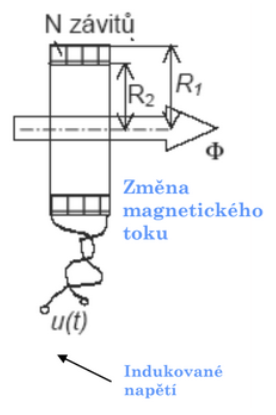
\includegraphics[scale = 0.4]{images/MerCivka.png}
\end{figure}

\subsection{Hallova sonda}
Využití Hallova jevu.\\
Sonda s polovodičovou destičkou.\\
Stejnosměrný proud I tekoucí v podélném směru.\\
Lorentzova síla - působí na pohybující se nosiče elektrického náboje v magnetickém poli. Jev spočívá ve vychylování směru toku el. Proudu v závislosti na velikosti indukce mag. Pole, které je kolmé na polovodičovou destičku.\\
\begin{figure}[h!]
    \centering
    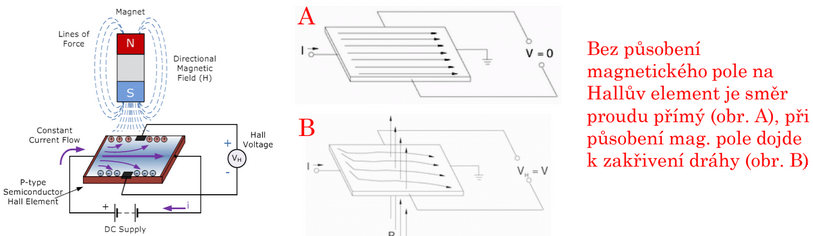
\includegraphics[scale = 0.5]{images/MVEHall1.png}
\end{figure}
\begin{center}
    \(u_H = \frac{R_H\cdot I}{d}\cdot B [V]\)
\end{center}
Kde \(R_H\) je Hallova konstanta \([m^3/C]\)

\begin{figure}[h!]
    \centering
    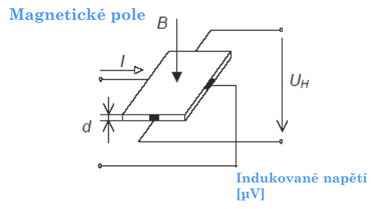
\includegraphics[scale = 0.5]{images/MVEHall3.png}
\end{figure}

\subsubsection{Charakteristika a použití}
\begin{itemize}
    \item Malé konsrukční rozměry
    \item Měření kolmé složky magnetické indukce ve vzduchových mezerách
    \item Měření nejsou ovlivňována, sonda nemá feromagnetické části
    \item Malý napájecí proud(10-100mA)
    \item Dobrá linearita převodní charakteristiky
    \item Meření stejnosměrných a střídavých magnetických polí nízkých kmitočtů
    \item Nevýhoda - teplotní závislost (kompenzace pomocí polovodičů s opačným teplotním koeficientem než má sonda)
\end{itemize}

\subsection{Feromagnetická sonda}
Nejrozšířenější typ magnetické sondy obsahuje 2 jádra. Má 2 feromagnetické jádra z kvalitního feromagnetického materiálu(měkký ferit) a ta jsou ovinuta stejným počtem závitů a umístěna do vnější cívky. Vinutí jader jsou zapojena proti sobě a napájena střídavým proudem.\\
Vlivem vnějšího stejnosměrného magnetického pole s intenzitou H, je souměrnost magnetický toků \(\Phi_1\) a \(\Phi_2\) porušena a na vnější cívce se indukuje napětí úměrné H.\\
\begin{figure}[h!]
    \centering
    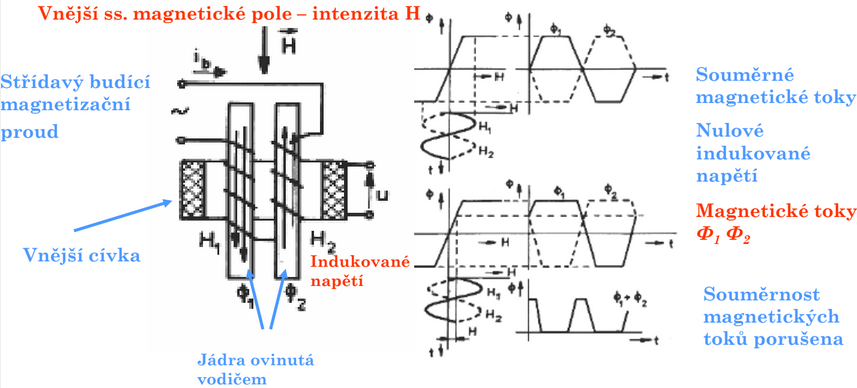
\includegraphics[scale = 0.5]{images/FeromagSonda.png}
\end{figure}
\subsubsection{Charakteristika a použití}
\begin{itemize}
    \item Měření velmi slabých magnetických polí - stejnosměrné nebo nízkofrekvenční střídavá pole.
    \item Měřící rozsah \(100pT\) až \(200\mu T\)
    \item Vysoká citlivost oproti Hallově sondě
    \item Měření kolísání magnetického pole země
    \item Magnetické kompasy v letadlech a lodích
    \item Hledání rudných ložisek a feromagnetických materiálů pod povrchem
    \item Indikace vad materiálů
\end{itemize}

\subsection{Rogowskiho-Chattockův potenciometr}
Potenciometr jako zvláštní úprava měřící cívky pro integrační měření.\\
Pásek z nemagnetického a nevodivého materiálu s konstantním průřezem rovnoměrně ovinutý po celé délce vodičem.\\
Změny magnetického toku \(\Phi\) v cívce -> vznik indukovaného impulsu napětí u(t).\\
Konstrukce: Měřící cívka pro integrační měření. Měření změn magnetického napětí \(U_m\).\\
\begin{figure}[h!]
    \centering
    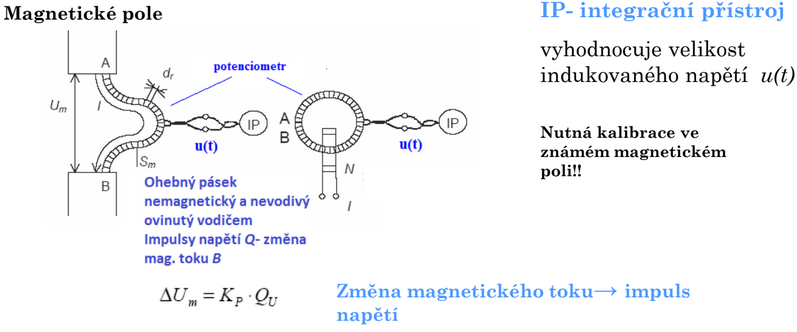
\includegraphics[scale = 0.5]{images/RChPoten.png}
\end{figure}

\subsection{Anizotropní magnetorezistor(AMR)}
Magnetorezistivita - změna odporu s magnetickým polem.\\
Anizotropní magnetorezistivita - změna odporu souvisí se změnou úhlu mezi vektorem magnetizace a směrem proudu, který protéká daným materiálem.\\
Princip: Změna elektrického odporu vlivem magnetického pole - dochází k ovlivňování nosičů náboje, což se projeví jako změna odporu materiálu. Vodivost feromagnetika ve směru magnetizace je menší než ve směru kolmém.\\
AMR efekt: elektrický opor ve směru magnetizace je vyšší než ve směru kolmém.\\
Provedení: tenká vrstva permalloye je nanesena na křemíkový substrát.\\
Remanentní magnetizace leží ve směru x (remanentní magnetizace je zbytková magnetizace, kterou si udrží feromagnetický materiál, když na něj přestane působit magnetické pole).\\
\begin{figure}[h!]
    \centering
    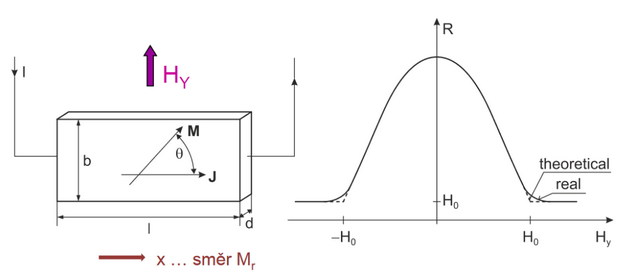
\includegraphics[scale = 0.5]{images/AMR.png}
\end{figure}

\(H_Y\) otáčí magnetizaci M a velikost R se mění o 2-3\%.\\
Senzor je tvořen tenkou vrstvou slitiny železa a niklu (permalloy). Pokud na senzor nepůsobí magnetické pole, má svůj klidový odpor. Působením magnetického pole tento klidový odpor klesá téměř lineárně(jen v rozsahu 2-3\%).\\
Použití:
\begin{itemize}
    \item Stejnosměrné i střídavé pole
    \item Měřící rozsah B od \(1\mu T\) do \(10mT\), v můstkovém uspořádání \(10nT\) až \(100\mu T\).
    \item Frekvenční rozsah DC až MHz
\end{itemize}
Vlastnosti: Závilost odporu na úhlu mezi proudem a magnetizací je silně nelineární.\\
Linearizace pomocí Barber poles struktury: Na pásek z permalloye jsou napařeny pod úhlem 45°proužky hliníku, který má výrazně vyšší vodivost než permalloy. Proud teče mezi hliníkovými proužky pod úhlem 45° k ose proužku, tím dochází k posunu charakteristiky. Tato technika vhodnější pro menší pole (kompas). \\
\begin{figure}[h!]
    \centering
    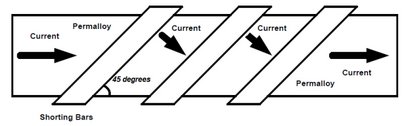
\includegraphics[scale = 0.7]{images/AMRLin.png}
\end{figure}

\subsection{Měření magnetizačních charakteristik materiálů}
\subsubsection{Vzorky}
Uzavřené:
\begin{itemize}
    \item Tvoří homogenní magnetický obvod s konstantním průřezem nepřerušený vzduchovou mezerou nebo s mezerou vyplněnou jiným materiálem
    \item Magnetický tok se uzavírá pouze feromagnetikem
    \item Výhoda - intenzita magnetického pole lze vypočítat z magnetizačního proudu, počtu závitů magnetizačního vinutí a střední délky siločar
\end{itemize}

Otevřené:
\begin{itemize}
    \item Obvykle tvar tyčí nebo pásků
    \item Magnetický tok se uzavírá vně vzorku vzduchem
    \item Intenzita magnetického pole se nedá určit výpočtem
    \item Obtížné dosažení homogenního rozložení toku v celém objemu vzorku
\end{itemize}
\begin{figure}[h!]
    \centering
    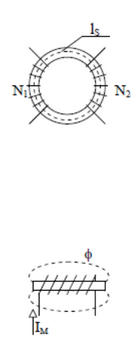
\includegraphics[scale = 0.6]{images/Vzorky.png}
\end{figure}

\subsubsection{Křivky}
Křivka prvotní magnetizace:
\begin{itemize}
    \item Výchozí stav - dokonalé odmagnetování
    \item Pomalu zvyšující se intenzita mag. Pole jedním směrem
    \item Nesmí nastat změna intenzity H opačného směru
\end{itemize}
Hysterezní křivka:
\begin{itemize}
    \item Vyjadřující závislost B = f(H) pro magnetizační cykly
    \item Změny intenzity mag. Pole → +H … -H
\end{itemize}
\begin{figure}[h!]
    \centering
    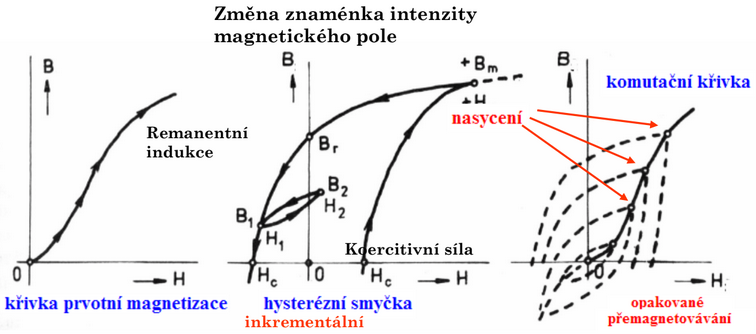
\includegraphics[scale = 0.5]{images/KrivkyMag.png}
\end{figure}

\subsubsection{Měření na uzavřených vzorcích}
\begin{figure}[h!]
    \centering
    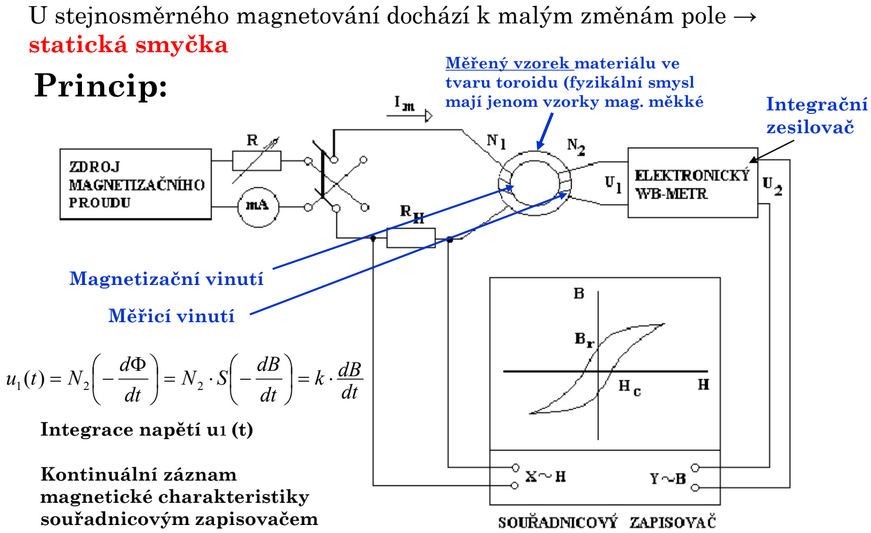
\includegraphics[scale = 0.5]{images/MerUzavVzor.png}
\end{figure}
Elektronický Wb-metr:
\begin{itemize}
    \item Tvořen integračním zesilovačem
    \item Nepříznicvě působí rušivá termoelektrická napětí ve vstupním obvodu. Kvůli tomu se používají vodiče a kontakty s malým termoelektrickým napětím.
    \item Rozsahy lze měnit přepínáním velikosti integračního rezistoru
\end{itemize}
\begin{figure}
    \centering
    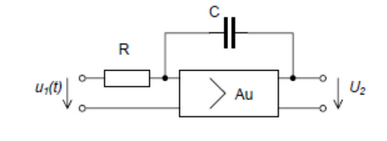
\includegraphics[scale = 0.9]{images/Wb-metr.png}
\end{figure}

\subsubsection{Měření na otevřených vzorcích}
Otevřené vzorky mají tvar válečku nebo kostky, jsou k dispozici častěji než prstencové vzorky.\\
Problém je správné určení intenzity magnetického pole, nelze ji odvodit z proudu jako u uzavřených vzorků -> pro magnetování se používá jha(ruční elektromagnet) z magneticky měkkého materiálu.\\
Postup:\\
\begin{itemize}
    \item Magnetické pole je buzeno magnetovacím vinutím \(N_1\) napájeným magnetovacím proudem ze zdroje Z.
    \item Tangenciální Hallova sonda (HS) slouží při určení intenzity H
    \item Magnetická indukce B se měří měřící cívkou s \(N_2\) závity pomocí fluxmetru F
\end{itemize}
Hysterezigrafy - přístroje jsou řízeny počítačem a proces měření je digitalizován.\\

\begin{figure}[h!]
    \centering
    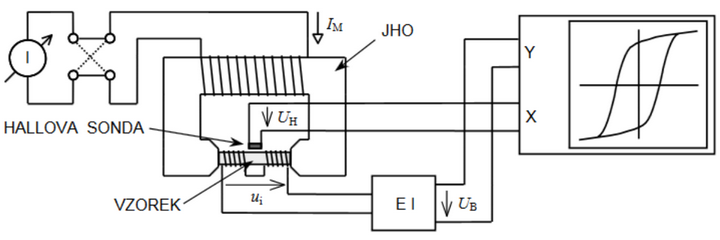
\includegraphics[scale = 0.5]{images/MerOtevVzor.png}
\end{figure}